\chapter{Radio Driver for Zolertia with the RN2483 module}

% Most of the LoRaWAN features were not implemented or tested since this was out of the scope of this project.

Since the \emph{Zolertia RE-Mote REV-B} don't support \emph{LoRa} out of the
box we have to implement a software driver for the Microchip \emph{RN2483} LoRa
module.

\section{Preliminary work}

Last year \emph{Roald Van Glabbeek} started to work on the \emph{RN2483} module
in the course of his master thesis~\cite{8847137} aiming on doing further
research on \emph{energy efficient lora multihop networks}.
For this purpose he created a \emph{RN2483 Shield} adapted to the pin
configuration of the \emph{Zolertia RE-Mote REV-B} and started a driver
implementation for the Contiki-OS\@.

In a previous attempt to adapt \emph{TSCH} for \emph{LoRa}
in~\cite{njomgang_2018}, Serge did his experimentation with the \emph{LoRaMote}
demo platform from \emph{Semtech} using a different LoRa radio module the
\emph{SX1272}. 
As analyzed in~\cite{8847137} the platform turned out to be an
issue because it was no longer produced, new versions were expensive and memory
was a bottleneck for further testing on the platform.
That's why \emph{Zolertia RE-Mote} was choosen. The platform is already available 
and well maintened in \emph{contiki-ng} (making the transition faster as less
code need to be developped) and the platform was already used in the \emph{ETRO Lab}.

The first part of my work consisted in implementing a reliable
and featurefull radio driver for the \emph{RN2483} module working in the last
version of \emph{contiki-ng}.

\section{RN2483 Module Structure}

Developped by \emph{Microchip} the \emph{RN2483} is a LoRa module working on
433 and 868Mhz band. The module is specically design to work with LoRaWAN
compliant network by including a set of commands specifically designed for
seamless connection with to a \emph{LoRaWAN} network. The module design is
aiming for ease of use over performance and low power.
All communication with the module are done with a \emph{UART} ASCII command
interface making it easy to interact with the module by a human that could be
entering command on a terminal and reading the response back in a human
readable format like in Fig~\ref{fig:pcconn}.

\begin{figure}[H] % TODO More info on axis
\centering
\begin{tikzpicture}[auto, thick]
  \node(pc) [server, label=below:{PC}] {};
  \node(ftdi) [draw, rectangle, right=of pc, right=4cm] {USB to UART Adapter};
  \node(module) [draw, rectangle, minimum size=6mm, right=of ftdi, right=2.5cm] (module) {RN2483 Module};

  \path (pc) edge[<->] node[]{USB Connection} (ftdi) ;
  \path (ftdi) edge[->,bend left] node[text width=1cm, align=center]{TX} (module);
  \path (module) edge[->,bend left] node[text width=1cm, align=center]{RX} (ftdi);
\end{tikzpicture}
\caption{Simple communication with the module scenario\label{fig:pcconn}}
\end{figure}


% Command type division
The module's interface include three types of cammands that enable access to
different functions.

\begin{itemize}
  \item \emph{radio} for the low-level radio commands to access the transceiver
    directly without the LoRaWAN interface.
  \item \emph{mac} for the LoRaWAN configurations and control. This command set
    will be used less as our implementation require low-level transceiver
    access.
  \item \emph{sys} for the module specific configurations such as the module
    GPIOs state, \emph{sleep}, EEPROM memory access, \ldots
\end{itemize}

\section{Testing Setup}

My testing setup was the same as~\cite{8847137}, I used a Zolertia RE-Mote
Rev-B platform, which is using a CC2538 microcontroller, and connected it to a
RN2483 breakout board in the same way as Fig~\ref{fig:schemaconn}. 
We are using the UART1 peripheral to communicate with the module because UART0
is used by the platform USB UART debbuger.

\begin{figure}[H]
  \centering
  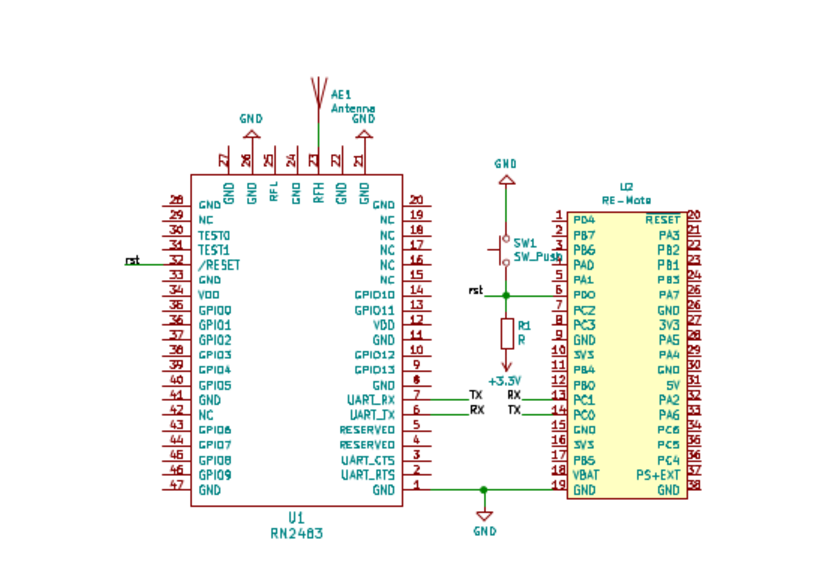
\includegraphics[scale=0.70]{thesis.tex/chapters/driver/fig/conn_diag.pdf}
  \caption{Hardware connection\label{fig:schemaconn}}
\end{figure}

\section{Implementation}

\subsection{Structure}

All the files for the driver implementation are available in
\lstinline{/arch/dev/rn2483} and examples are located in
\lstinline{/examples/platform-specific/rn2483}.
My implementation structure was inspired by the work in~\cite{8847137} and the
\emph{RIOT-OS} project\footnote{\url{https://github.com/RIOT-OS/RIOT}} which
already took care to define a lot of the parameters we want to use with the
module.

\begin{description}
  \item[lora] LoRa radio specific function, declaration and configuration. This
    include the function used to calculate the time on air as well as
    configuration structure and parameters.
  \item[rn2483-include] This file contain the declaration both needed by
    \lstinline{rn2483-uart} and \lstinline{rn2483} to avoid cycling inclusion
    that mess with the compiler.
  \item[rn2483-uart] Lower level implementation of the function to directly
    communicate with the module via UART\@. This part is the closest one to the
    hardware because of the uart implementation being specific to the CC2538.
  \item[rn2483-api] Complete coverage of the RN2483 commands. Using functions
    from this file allow the user of the driver to not bother with writting
    each command by hand and use a standardized structure instead.
  \item[rn2483] Implementation of the Contiki radio device driver. The file
    contain the standardized way of Contiki to use and configure a radio device.
    This is the structure shared by all the radio driver in Contiki.
\end{description}

\subsection{Synchronous communication with the module}

The first design challenge of the driver implementation is to create a
synchronous mechanism to receive message from the UART\@. 
The need for synchronous messaging is crucial when using this module, every
commands and configuration of the module is done via UART and a simple
acknowledgement from the command is almost mandatory to avoid two command
to clash by using the module at the same time.
The previous implementation in~\cite{8847137} used synchronous fixed delays to 
wait for the module response but this method has its own limitation 
as each commands has their own delays.

The UART driver implementation for the CC2538 don't have a synchronous blocking
read call for the UART out of the box and assume the programmer will use
response in processes instead. The way the receiption is working is by executing a 
so called \emph{input handler} at each interruption triggered from an 
UART reception.
The default input handler is the \lstinline{serial_line_input_byte} 
specifically designed for serial communication with a terminal and we will keep
using this handler with UART0 to get debug messages with a USB connection from 
a computer.
We have to define our own handler for UART1 peripheral to communicate with the
module.
It will be similar as the default one because they are both using same message
structure, terminating by \lstinline{\r\n} but 
where \lstinline{serial_line_input_byte} is passing each character to a standalone
process (\lstinline{serial_line_process}) broadcasting an event at command
reception, our handler is directly threating  the message in the interrupt.

Working with processes and events, is not possible in our use case because Contiki 
don't have any mechanisms allowing programmers to wait for an event inside a 
function. We can only wait for a specific event inside a process but doing 
everything inside a big process is not an option.
Our custom handler is designed as a state machine (Fig~\ref{fig:cmdstate}) and 
work with its own reception buffer. It takes advantage of the limited response 
format from the RN2483 module to sort each new communications.

\begin{itemize}
  \item Messages starting with \lstinline{radio rx  } are asynchronous LoRa
    messages.
  \item \lstinline{radio_tx_ok} indicate the end of a transmission. This
    implies we have done a transmission before.
  \item \lstinline{ok} indicate the acknowledgement of a command.
\end{itemize}

% Talk about the state machine

I implemented an helper functions, to ease the command transmission and
acknowledgement with the module.

\begin{description}
  \item[rn2483\_receive\_synch] busywait on the command states
    (Fig~\ref{fig:cmdstate}) until the received state or after the timeout
    passed.
  \item[rn2483\_send\_cmd] a printf style command with automatic wait
    for acknowledgement (with the possibility to add a custom timeout).
  \item[rn2483\_raw\_cmd] sending the command from a buffer without
    format or wait for acknowledgement.
\end{description}

\begin{figure}[H]
\centering
  \begin{tikzpicture}[->,>=stealth',shorten >=1pt,auto,node distance=3.5cm]
  \tikzstyle{every state}=[thick,draw=gray!50,fill=gray!20,draw=none,text=black]

  \node[initial,state] (A)                    {Transmission};
  \node[state]         (B) [above right of=A] {Reception};
  \node[state]         (C) [below of=B]       {Timeout};
  \node[state]         (D) [right of=B]       {Received};

  \path (A) edge [bend right]    node {     } (B)
            edge [bend left]     node {     } (C)
        (B) edge [bend left]     node {     } (C)
            edge                 node {     } (D)
        (C) edge [bend left]     node {     } (A)
        (D) edge [bend right=85] node {     } (A);
\end{tikzpicture}
\caption{The command states\label{fig:cmdstate}}
\end{figure}


\subsection{Transmission}

The radio transmission command has a different pattern from the other commands 
available for the module. After the acknowledgement of the radio transmission 
command the module will send another message once the message is fully
transmitted.

\begin{figure}[H]
\centering

\begin{sequencediagram}

\newthread{A}{RE-Mote}{}
\newinst[1]{B}{RN2483}{}
\newinst[3]{C}{Radio Band}{}
\begin{call}{A}{radio tx~\ldots}{B}{radio\_tx\_ok}
  \messdash{B}{ok}{A}
  
  \begin{sdblock}{Radio Transmission}{Transmition time calculated
    in~\ref{eq:tpacket}}
    \begin{call}[4]{B}{}{C}{}
    \end{call}
  \end{sdblock}
\end{call}

\end{sequencediagram}

  \caption{\lstinline{radio tx} command sequence diagram\label{fig:txsequence}}

\end{figure}



Microchip chose to represent the payload as string formated hex number to
facilitate the manual writing of commands, making the message paylaod twice as
long as its original content. As all the content we will handle 
are represented as \emph{8 bit} number array, a function to convert array to
string representation and vice versa was taken from the RIOT-OS project.

\subsection{Asynchronous Reception}

The last component of a complete driver implementation is to receive radio
messages.
Reception follow a different scheme from the other commands because a message
reception can happen at any time asynchronously from the moment we run the
command \lstinline{radio rx 0}.
To tackle this issue a one message inbox was implemented (see
Fig~\ref{fig:rxstate}).
When a command is fully transmitted from the module we look at the structure of
the message. Every message received from the radio start with \lstinline{radio rx  }, if it follow this structure a flag is set and is unset at the moment we
read the message from our code.
Messages are received in a string formated hex number and we convert it to and \emph{8
bit integer array}. This array is stored in a different place than the received
message as command may be executed between the moment we receive the message and
the moment we read it.
Also a timestamp is saved at the reception to keep track of when was received the
message.

\begin{figure}[H]
\centering
  \begin{tikzpicture}[->,>=stealth',shorten >=1pt,auto,node distance=3.5cm]
  \tikzstyle{every state}=[thick,draw=gray!50,fill=gray!20,draw=none,text=black]

  \node[initial,state] (A)              {None};
  \node[state]         (B) [right of=A] {Received};

    \path (A) edge [bend right] node[below] {Reception} (B)
          (B) edge [bend right] node[above] {Read} (A);
\end{tikzpicture}
\caption{The RX states\label{fig:rxstate}}
\end{figure}


\subsection{Contiki Radio Driver}

\section{Validation test}

% Talk about project configuration like with the NETSTACK
